\documentclass{article}

\usepackage[utf8]{inputenc} % use UTF-8
\usepackage[T2A,OT1]{fontenc} % rus fonts
\usepackage[russian]{babel}

\usepackage{tikz}
\pagenumbering{gobble}
\usepackage{geometry}
\usepackage{subfigure}
\usepackage{hyperref}

% web links style
\usepackage{hyperref}
\hypersetup{
	colorlinks=true,
	linkcolor=blue,
	urlcolor=blue,
}

\geometry{
	a4paper,
	total={175mm,257mm},
	left=20mm,
	top=20mm,
	bottom=0mm,
}

\urlstyle{same}


\begin{document}
	\section*{ПРОФИЛИРОВАНИЕ JAVA ПРИЛОЖЕНИЯ}
	\subsection*{Праметры системы}
	\begin{tabular}{ll}
		Название      & Значение                                  \\
		ПК            & Lenovo ThinkPad T570                      \\
		Процессор     & Intel(R) Core(TM) i5-7200U CPU @ 2.50GHz  \\
		ОЗУ           & 8192 MB DDR4 @ 2133 MHz                   \\
		OC            & 16.04.1-Ubuntu x86\_64                     \\
		Java          & Java(TM) SE Runtime Environment (build 1.8.0\_144-b01) \\
		JVM           & Java HotSpot(TM) 64-Bit Server VM (build 25.144-b01, mixed mode) \\
		JMC           & 5.5.1                                     \\
		jmap          & из JDK 1.8.0\_144                          \\
		maven          & 3.3.9                                     \\
	\end{tabular}

	\subsection*{Репозиторий}
		В репозитории  \href{https://github.com/eremeykin/hh-jvm/}{hh-jvm} есть четыре ветки:
		\begin{itemize}
			 \item \texttt{master} - ветка исходного репозитория \href{https://github.com/yarkinsv/money-transfer}{money-transfer}
			 \item \texttt{automation} - ветка автоматизации профилирования, тут созданы файлы \texttt{profile.sh} скрипт автоматизирующий профилирование,
			  \texttt{flight-recorder.jfc} файл с настройками для FlightRecorder и \texttt{analyze.py} файл для анализа вывода скрипта \texttt{run\_tests.py}
			 \item \texttt{develop} - ветка с изменениями в java коде для улучшения производительности.
			 \item \texttt{report} - ветка с отчётом			 
		\end{itemize}

		Стадии экспериментов помечены тегами \texttt{stage\_<\#стадии>}. Дампы памяти и записи параметров на github не выложены, они знимают много места.


	\subsection*{Стадии экспериментов}
		Эксперименты проводятся в несколько стадий, каждая стадия отличается от предыдущей изменениями в коде и на каждой стадии снимаются показатели производительности текущей версии кода. Всего есть 3 стадии :
		\begin{itemize}
			\item  Стадия 0 (тег \texttt{stage\_0}): код без изменений. На этой стадии выделяются основные ошибки, которые удается найти с помощью профилировщика.
			\item Стадия 1 (тег \texttt{stage\_1}): код содержит исправления, найденные на предыдущей стадии, а также при инспекции кода
			\item Стадия 2 (тег \texttt{stage\_2}): реализация DAO переписана, хранение реализовано на \texttt{HashMap}.
		\end{itemize}

	\subsection*{Инструменты}
		Для замеров используются следующие инструменты:
		\begin{itemize}
			\item Cамописный bash скрипт \texttt{profile.sh} для автоматизации замеров и обеспечения некоторой степени воспроизводимости экспериментов.
			\item Cамописный python скрипт \texttt{analyze.py} для построения графика времени выполнения сценария 1.
			\item \href{https://docs.oracle.com/javacomponents/jmc-5-5/jfr-runtime-guide/about.html}{FlightRecorder} для записи \texttt{jfr} файлов с различными измеряемыми параметрами, перечисленными в файле \texttt{flight-recorder.jfc}
			\item \href{https://www.oracle.com/technetwork/java/javaseproducts/mission-control/index.html}{Java Mission Control} для анализа \texttt{jfr} файлов. Файлы \texttt{jfr} объемные и в репозиторий не входят.
			\item \href{https://docs.oracle.com/javase/8/docs/technotes/tools/unix/jmap.html}{jmap} для сохранения бинарный дампов памяти. Дампы большие, в репозиторий не входят.
			\item \href{https://docs.oracle.com/javase/8/docs/technotes/guides/visualvm/index.html}{jvisualvm} для анализа дампов памяти и фильтарции объектов по пакету
		\end{itemize}
	
	\subsection*{Замеряемые величины}
	Согласно заданию, требуется контролировать следующие параметры:
		\begin{itemize}
			\item На сколько загружен CPU - оценивается по записям FlightRecorder
			\item Сколько в среднем потребляется памяти, заметен ли в программе memory leak - оценивается по записям FlightRecorder
			\item Как часто происходит сборка мусора - оценивается по записям FlightRecorder, тут же оцениваются дампы памяти \texttt{.hprof} с помощью jvisualvm
			\item Сколько в среднем выполняется запуск сценария 1, как быстро увеличивается это время - оценивается по графику, построенному с помошью \texttt{analyze.py} 
			\item Какие операции из значимых (т.е. без учёта работы системных функций, в т.ч. веб сервера) занимают больше всего процессорного времени - оценивается по записям FlightRecorder
		\end{itemize}
	
	\subsection*{Методика}
	В \texttt{run\_test.py} добавлен вывод прошедшего с момента запуска времени, этот вывод мы будем перенаправлять в файл \texttt{.plg} (python log) и потом анализировать.
	На каждой стадии запускаем самописный \texttt{profile.sh} скрипт командой
	\texttt{./profile.sh -{}-clear \&\& ./profile.sh -{}-dump \&\& sleep 30 \&\& ./profile.sh}

		\begin{itemize}
			\item \texttt{./profile.sh -{}-clear} --- чистит старые дампы и \texttt{jfr} файлы и делает texttt{mvn clean install}
			\item \texttt{./profile.sh -{}-dump} --- запускает jar-ник и раз в 2 мин делает дамп через texttt{jmap} в течении 10 мин
			\item \texttt{./profile.sh} --- записывает \texttt{jfr} файл в течении 10 мин с помощью FlightRecorder и JMC .
		\end{itemize}

	Таким образом, сохранение дампов и запись jfr файлов происходит на разных запусках jar-ника.

	После выполнения скрипта получаем файлы:
		\begin{itemize}
			\item два \texttt{jfr} файла --- один тот, в процессе записи которого не создавались дампы, а второй записывался одновременно с созданием дампов. Для анализа интересен первый
			\item два \texttt{plg} файла --- файлы output потока python скрипта \texttt{run\_test.py}, в который ещё добавлено время для каждой итерации. Один во время "чистого" прогона, а второй во время сохранения дампов памяти. Интересен первый. 
			\item 5 дампов памяти, так как их пишем через каждые 2 мин в течении 10 минут . Анализируем средний, третий, созданный через 6 мин после начала записи.
		\end{itemize}
	Полученные файлы анализируются с помощью jvisualvm (для дампов) и JMC (для \texttt{jfr}), 
	а также самописным python скриптом \texttt{analyze.py} (для построения графика времени выполнения сценария 1 по \texttt{plg} файлу)


	\section*{Стадия 0}
	Анализ производительности приложения до изменений кода.
	\begin{itemize}
		\item Выясняется, что сохранение дампов во время работы практически не сказывается на производительности, поэтому на самом деле можно запускать один раз на 10 мин \texttt{./profile.sh --dump}, вместо того чтобы за первый проход собирать дампы, а за второй писать события FlightRecorder'ом.
		\newpage
		\item \textit{На сколько загружен CPU?}
		
		Анализируем загрузку CPU из записанного \texttt{jfr} файла. Она в среднем составляет 23\%. 
		\begin{figure}[h!] % \ContinuedFloat
			\centering
			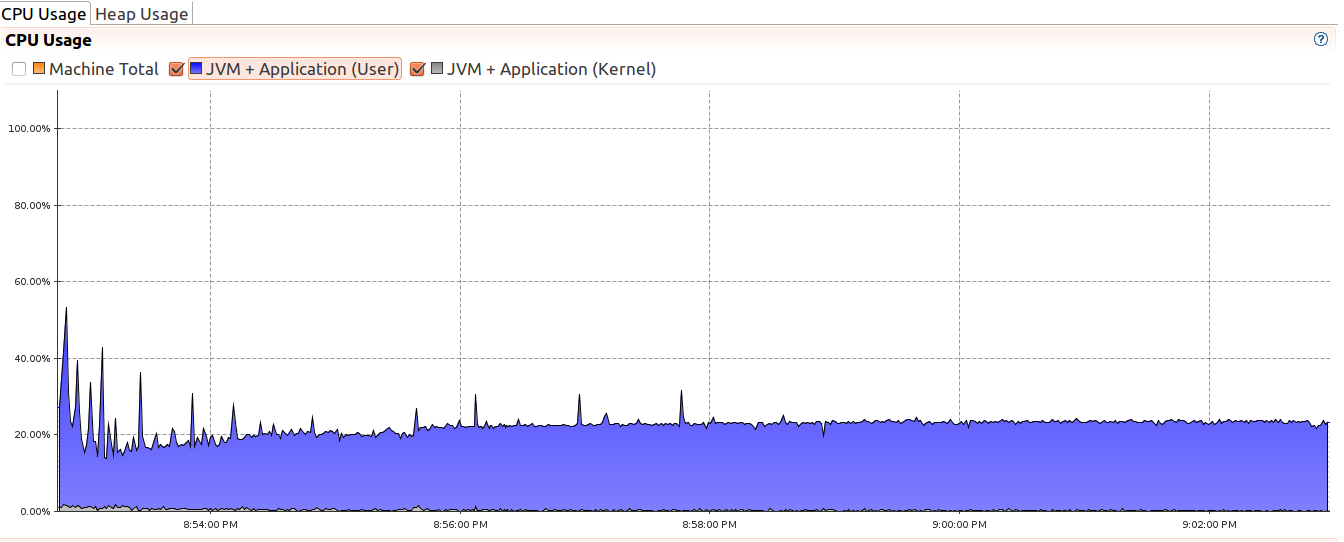
\includegraphics[width=0.95\linewidth]{img/stage_0/cpu.png}
	%		\caption{Test}
			\label{fig:cpu0}
		\end{figure}
		
		\item \textit{Сколько в среднем потребляется памяти, заметен ли в программе memory leak?		}

		Использование heap от 50 Мб до 145Мб:
		\begin{figure}[h!] % \ContinuedFloat
			\centering
			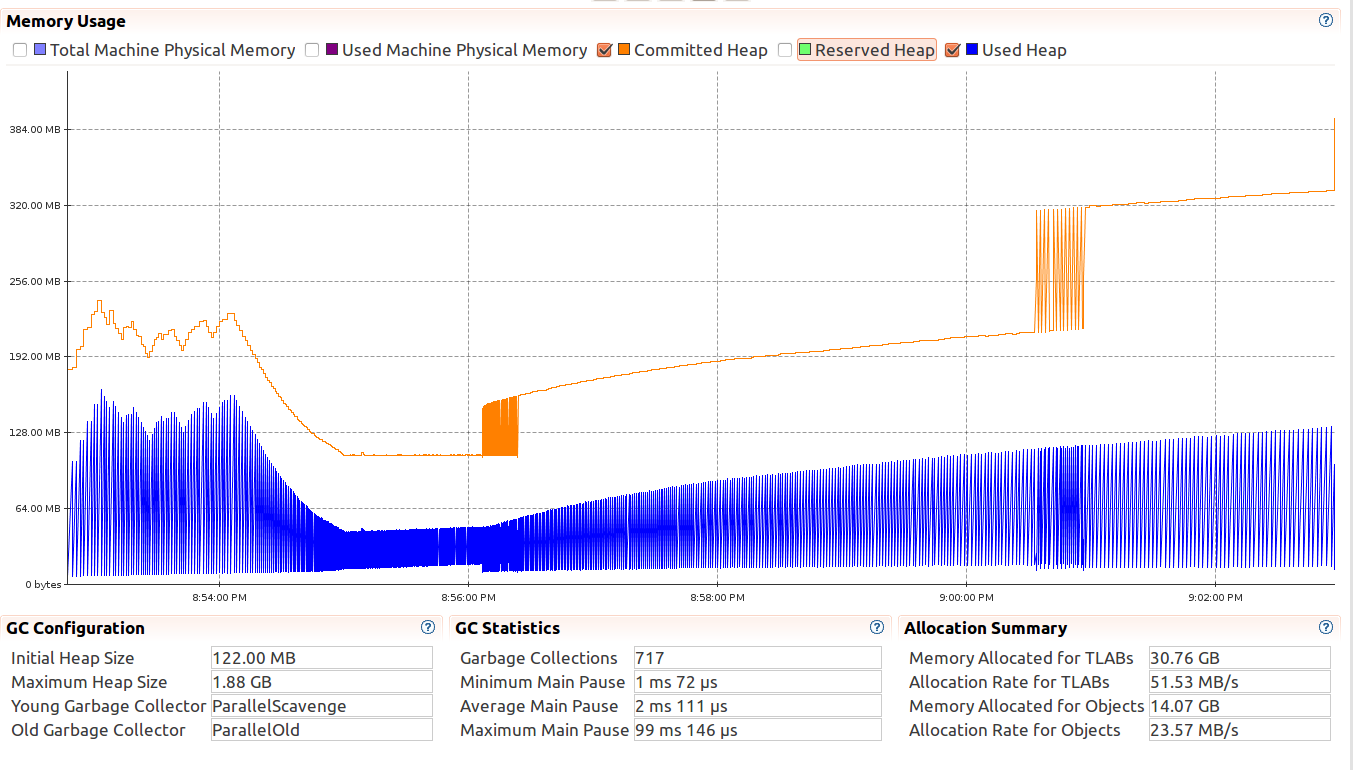
\includegraphics[width=0.95\linewidth]{img/stage_0/memory.png}
			%		\caption{Test}
			\label{fig:mem0}
		\end{figure}
		\newpage

		Дамп \#3
		\begin{figure}[h!] % \ContinuedFloat
			\centering
			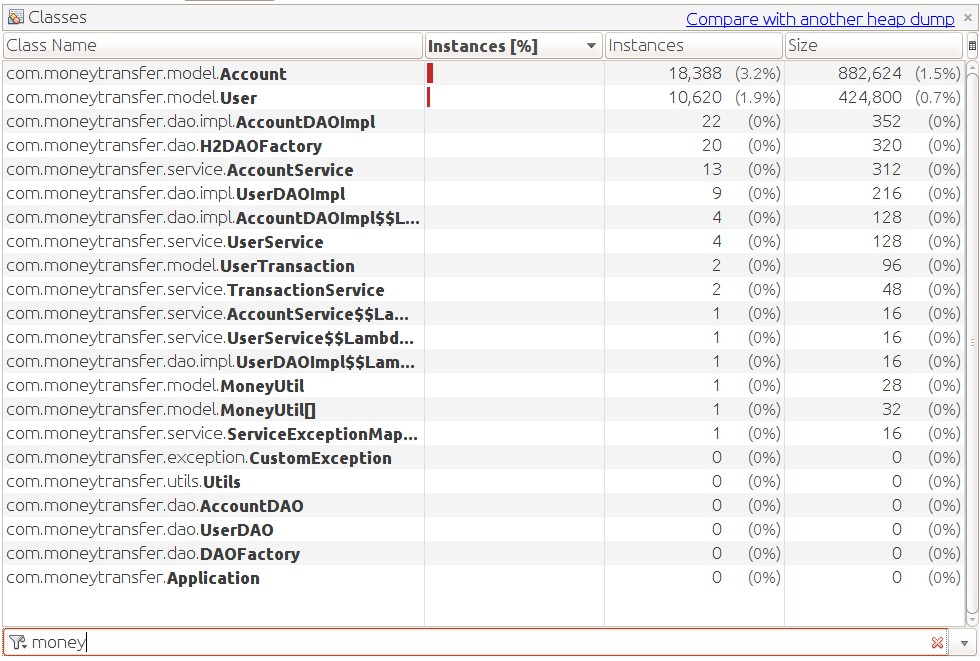
\includegraphics[width=0.75\linewidth]{img/stage_0/dump3.png}
			%		\caption{Test}
			\label{fig:dmp30}
		\end{figure}
		
		Относительно много объектов \texttt{Account} и \texttt{User}, почему-то создано несколько объектов типа \texttt{DAOImpl}. 
		
		\item \textit{Как часто происходит сборка мусора?}
		
		За время эксперимента (10мин 11с) произошла 717 раз. Средняя пауза 2 ms 111 us, максимальная 99 ms 146 us. 
		
		\item \textit{Сколько в среднем выполняется запуск сценария 1, как быстро увеличивается это время?}
		
		На графике показано среднее время \texttt{Execution time average} и текщее время \texttt{Execution time last} в секундах зависимости от числа выполнения сценария 1 \texttt{Function play\_scenario\_1 called}. 
		Текущее время выросло с 0.03 с до  0.4 с за 3850 выполнений сценария.
		
		\begin{figure}[h!] % \ContinuedFloat
			\centering
			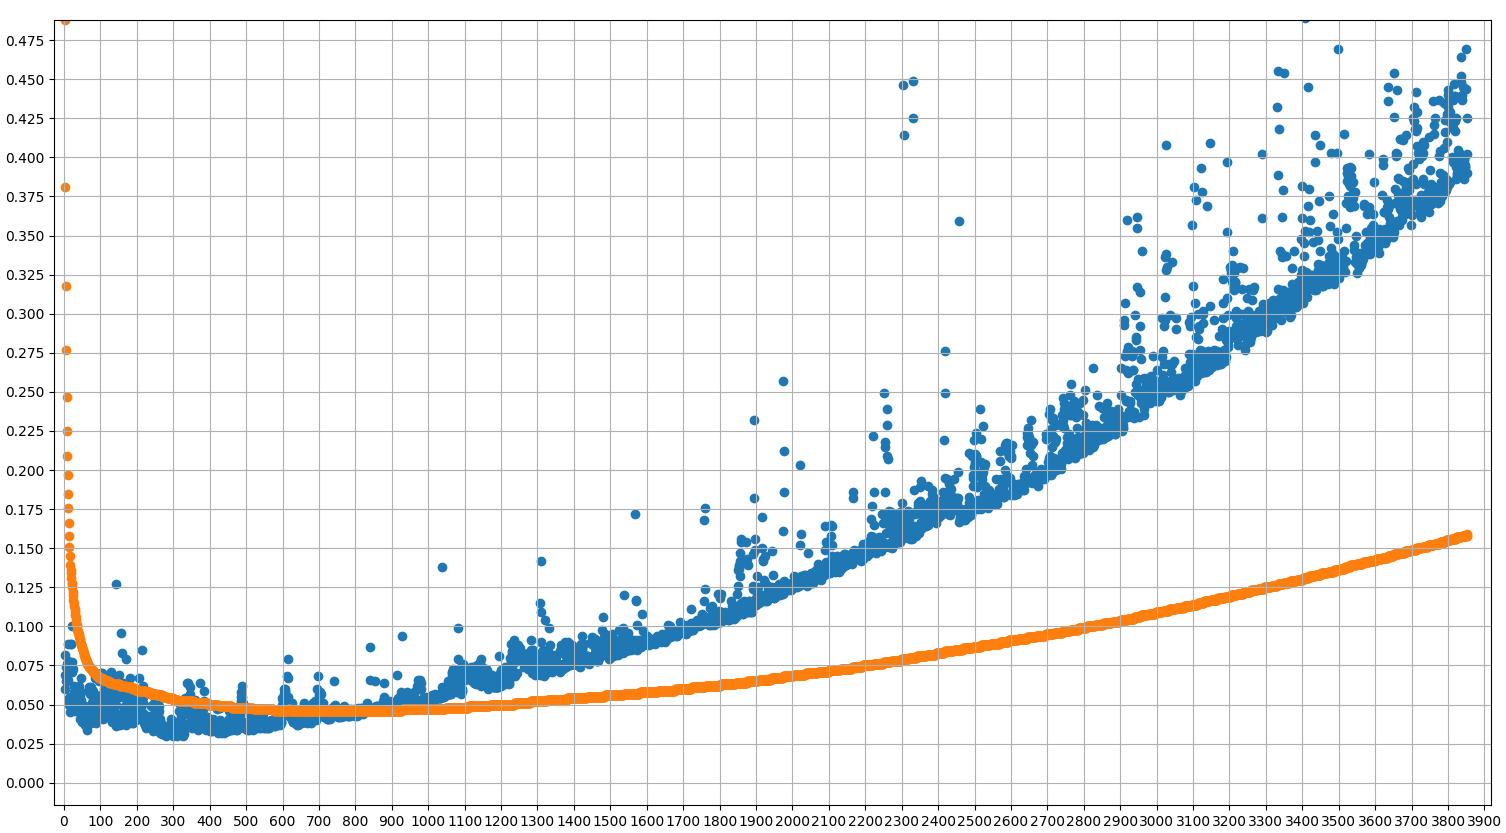
\includegraphics[width=0.95\linewidth]{img/stage_0/pyplot.png}
			\label{fig:pyplot0}
		\end{figure}
		
		\newpage
		\item \textit{Какие операции из значимых (т.е. без учёта работы системных функций, в т.ч. веб сервера) занимают больше всего процессорного времени?}

		Семплирование, применённое при записи, имеет ограниченную точность и общее число вызова значимых функций не велико, 
		в основном процессор выполняет функции из jdk или веб сервера, но оценить узкие места можно при помощи таблицы: 

		\begin{figure}[h!] % \ContinuedFloat
			\centering
			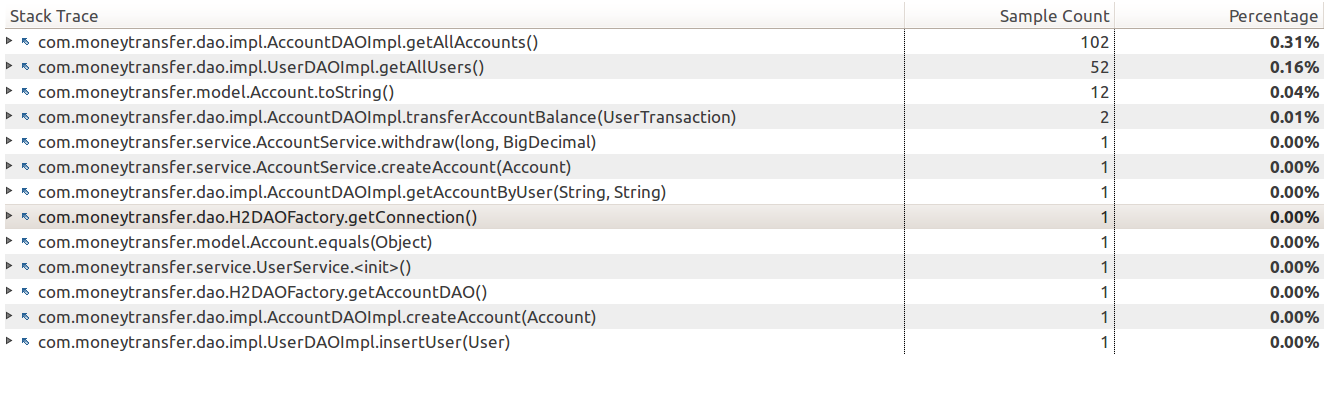
\includegraphics[width=0.95\linewidth]{img/stage_0/hotmethods.png}
			\label{fig:hotmethods0}
		\end{figure}

		\item \textbf{ВЫВОДЫ СТАДИИ 0}
		\begin{enumerate}
			\item Проверить как создаются и куда сохраняются объекты \texttt{Account} и \texttt{User}.
			\item Проверить почему создаётся несколько объектов типа \texttt{*DAOImpl} и \texttt{H2DAOFactory}
			\item Проверить вызов методов \texttt{AccountDAOImpl.getAllAccounts()}, \texttt{UserDAOImpl.getAllUsers()}
		\end{enumerate}
	\end{itemize}





	\section*{Стадия 1}
		При анализе найдено, что
	\begin{enumerate}
		\item \texttt{9b81cd4} В классе есть \texttt{UserDAOImpl} есть неиспользуемое поле \texttt{fatched} 
		\item \texttt{fa418f8} Объекты типа \texttt{DAO} можно переиспользовать, не создавая заново новые объекты, так как они не имеют состояния 
		\item \texttt{501dd00} В классе \texttt{UserTransaction} в методе \texttt{equals()} можно переупорядочить порядок сравнения полей
		\item \texttt{e9eed2d} Обнаружена ещё одна утечка памяти, экземпляры \texttt{Pattern} можно переиспользовать
		\item \texttt{d78be31} В методах \texttt{getDAO} можно убрать \texttt{loadDriver}
		\item \texttt{42a5108} В классе \texttt{Account} \texttt{hashCode} возвращал константу
		\item \texttt{d6ee875} В методе \texttt{getAccountByUser()} неправильно возвращается значение
		\item \texttt{9cb79c3} В таблице \texttt{User} можно установить \texttt{AUTO\_INCREMENT} и возвращать значение, сгенерированное базой данных
		\item \texttt{83dd1f1} Можно переиспользовать объекты \texttt{H2DAOFactory}
		\item \texttt{68a205b} Переписаны методы \texttt{getAllAccounts} и \texttt{getAllUsers} для использования \texttt{StringBuilder} (не уверен, не будет ли старая реализация создавать и соединять лишние строки)
	\end{enumerate}		


	\newpage

	\begin{itemize}
		
		\item \textit{На сколько загружен CPU?}
		
		Загрузка ЦП уменьшилась до 15\% в среднем.
		\begin{figure}[h!] % \ContinuedFloat
			\centering
			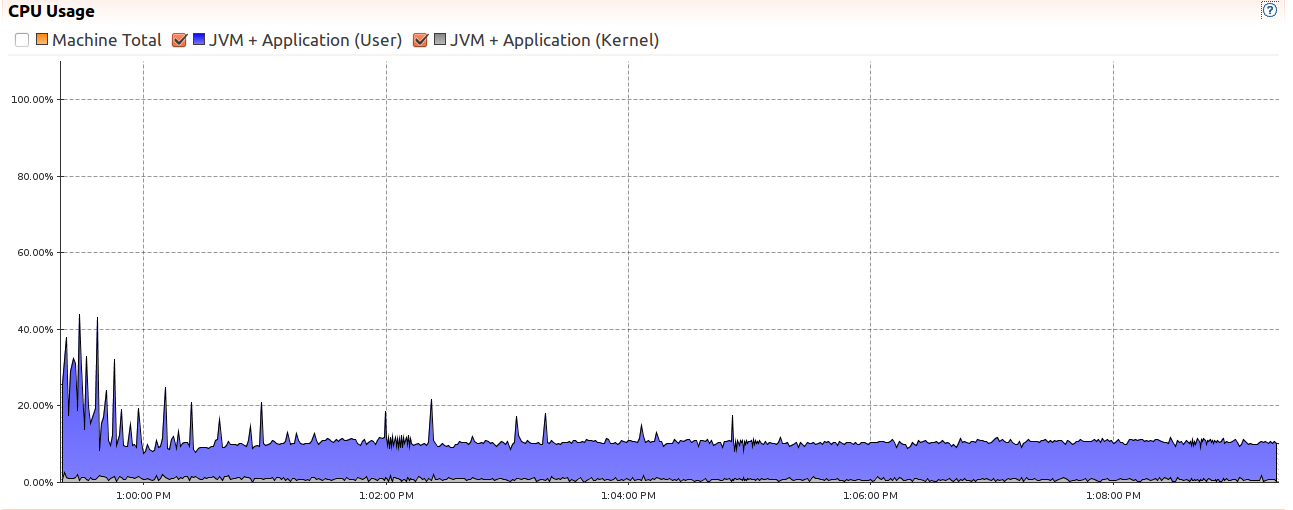
\includegraphics[width=0.95\linewidth]{img/stage_1/cpu.png}

			\label{fig:cpu1}
		\end{figure}
		
		\item \textit{Сколько в среднем потребляется памяти, заметен ли в программе memory leak?		}
		
		Использование heap составляет от 50 Мб до 400Мб:
		\begin{figure}[h!] % \ContinuedFloat
			\centering
			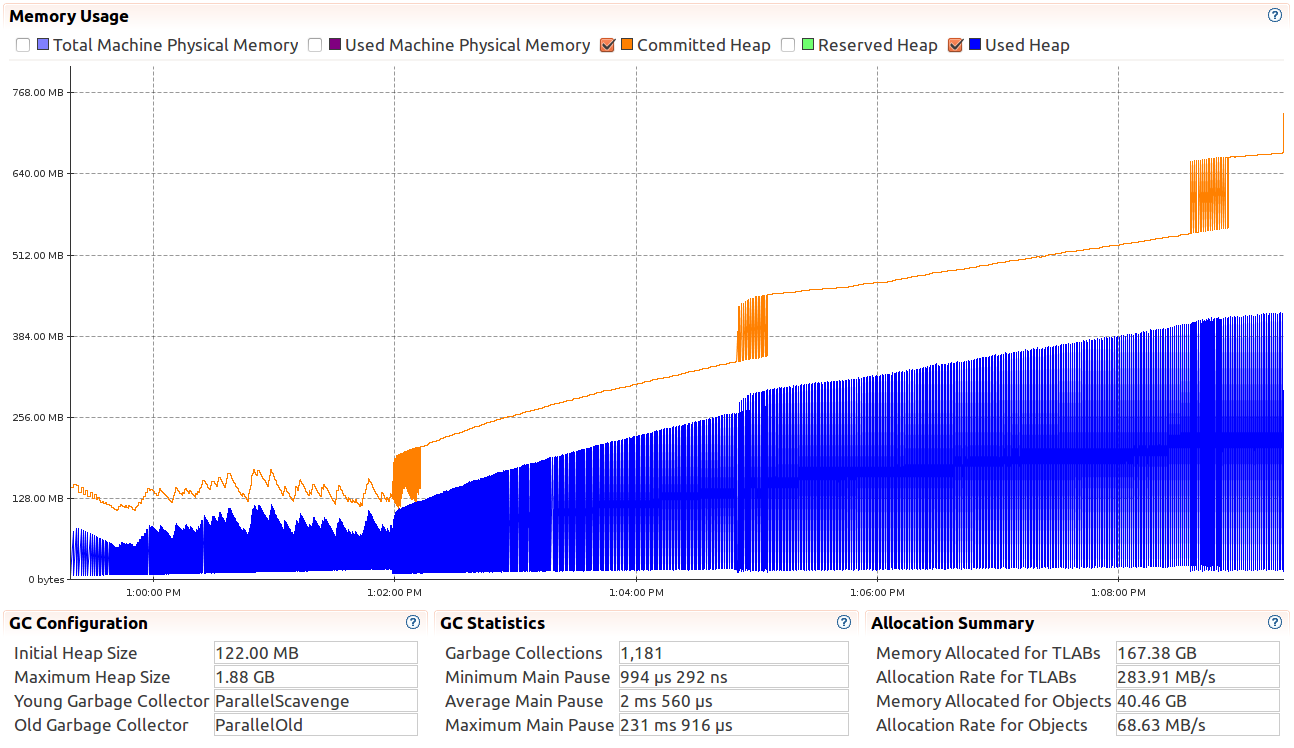
\includegraphics[width=0.95\linewidth]{img/stage_1/memory.png}
			%		\caption{Test}
			\label{fig:mem1}
		\end{figure}
		\newpage
		
		Дамп \#3
		\begin{figure}[h!] % \ContinuedFloat
			\centering
			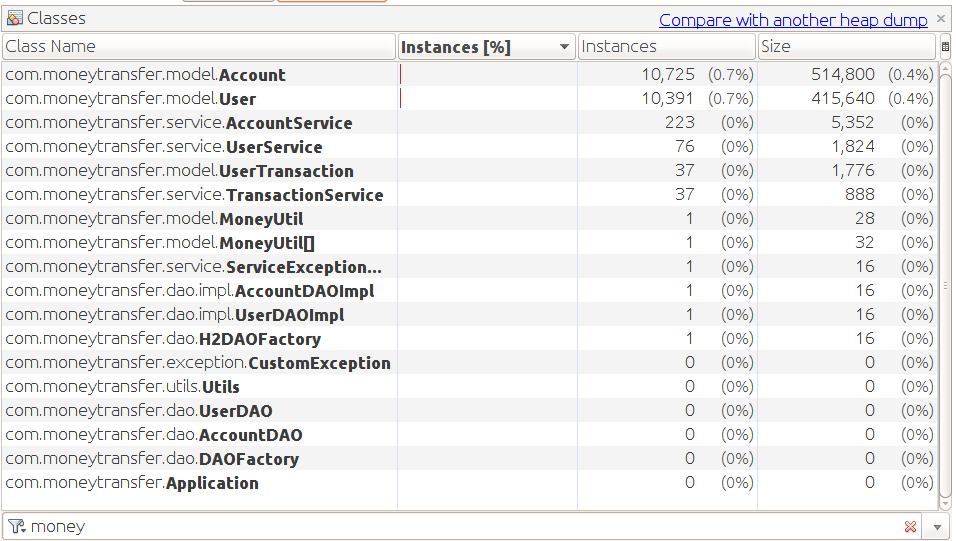
\includegraphics[width=0.75\linewidth]{img/stage_1/dump3.png}
			%		\caption{Test}
			\label{fig:dmp31}
		\end{figure}
		
		Число объектов сократилось, но не радикально, такие изменения могут быть вызваны временем
				
		\item \textit{Как часто происходит сборка мусора?}
		
		За время эксперимента произошла 1181 раз. Средняя пауза 2 ms 560 us, максимальная 231 ms 916 us. 
		
		\item \textit{Сколько в среднем выполняется запуск сценария 1, как быстро увеличивается это время?}
		
		Текущее время выросло с 0.035 с до  0.48 с за 11300 выполнений сценария 1. 
		Таким образом, производительность существенно возросла. На предыдущей стадии 0 сценарий 1 был выполнен всего 3850 раз. 
		Рост времени выполнения сценария 1 существенно более медленный.
		
		\begin{figure}[h!] % \ContinuedFloat
			\centering
			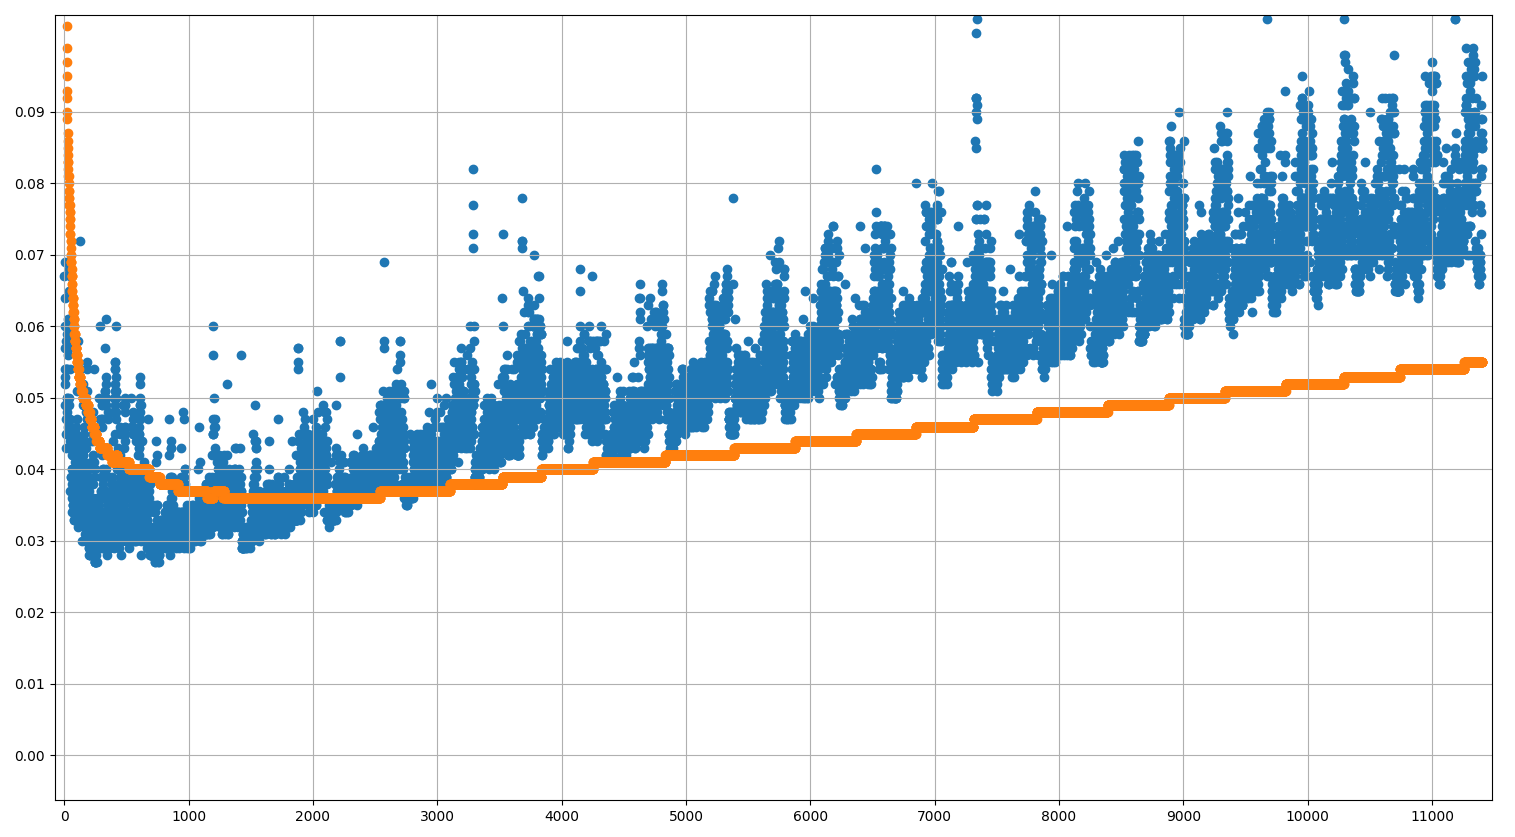
\includegraphics[width=0.95\linewidth]{img/stage_1/pyplot.png}
			\label{fig:pyplot1}
		\end{figure}
		
		\newpage
		\item \textit{Какие операции из значимых (т.е. без учёта работы системных функций, в т.ч. веб сервера) занимают больше всего процессорного времени?}
		
		Статистика использования методов изменилась не сильно, возможно она зависит только от характера загрузки сервера.
		
		\begin{figure}[h!] % \ContinuedFloat
			\centering
			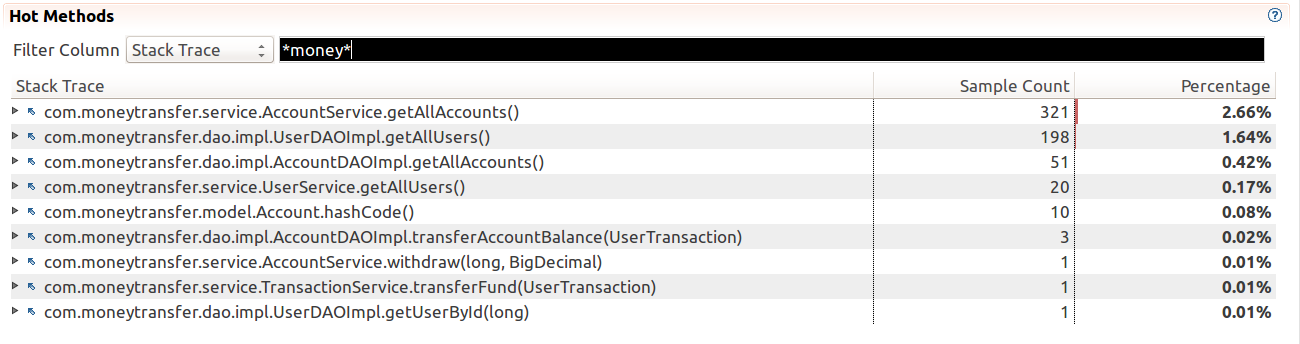
\includegraphics[width=0.95\linewidth]{img/stage_1/hotmethods.png}
			\label{fig:hotmethods1}
		\end{figure}
		
		\item \textbf{ВЫВОДЫ СТАДИИ 1}
		\begin{enumerate}
			\item Загрузка процессора снизилась с 25\% до 15\%.
			\item Потребление памяти увеличилось 50--145 Мб до 50--400 Мб, возможно это связано с общим ростом производительности, а не с утечкой памяти. Мне не удалось найти больше кода, который мог бы вызывать утечку памяти. 
			Анализ дампов также не проясняет этот вопрос.
			\item Общая производительность существенно возросла согласно результатам замера времени выполнения сценария 1.
		\end{enumerate}
	\end{itemize}
	

\section*{Стадия 2}

\begin{enumerate}
	\item \texttt{9b81cd4} В классе есть \texttt{UserDAOImpl} есть неиспользуемое поле \texttt{fatched} 
\end{enumerate}		


\begin{itemize}
	
	\item \textit{На сколько загружен CPU?}
	
	Загрузка ЦП уменьшилась до $ \sim12\%  $в среднем.
	\begin{figure}[h!] % \ContinuedFloat
		\centering
		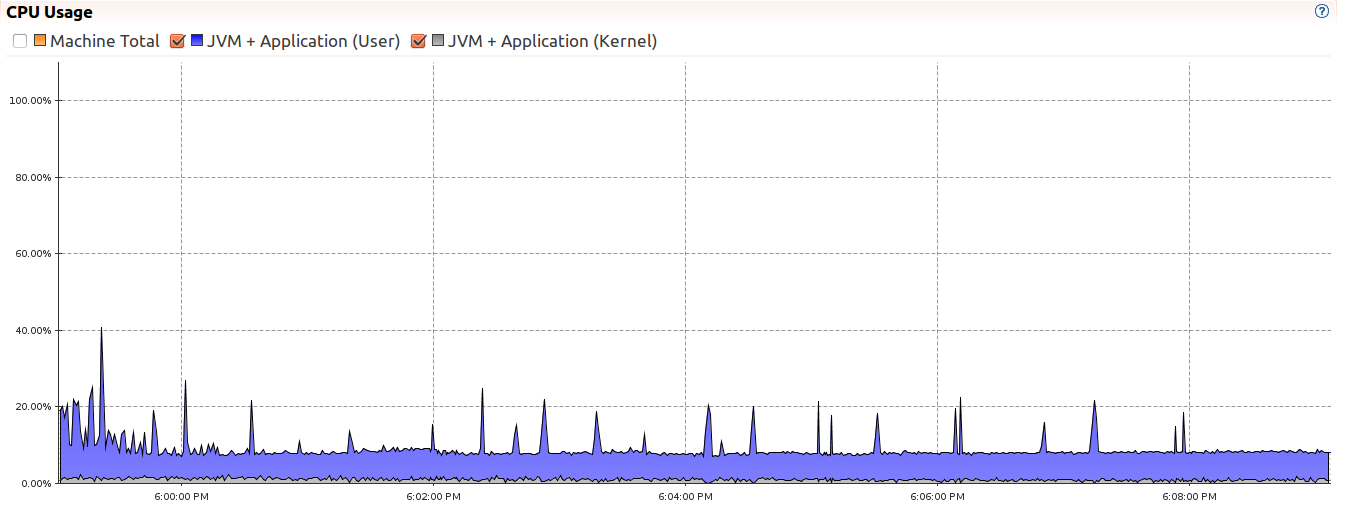
\includegraphics[width=0.95\linewidth]{img/stage_2/cpu.png}
		
		\label{fig:cpu2}
	\end{figure}
	
	\item \textit{Сколько в среднем потребляется памяти, заметен ли в программе memory leak?}
	
	Использование heap составляет от 50 Мб до 370Мб:
	\begin{figure}[h!] % \ContinuedFloat
		\centering
		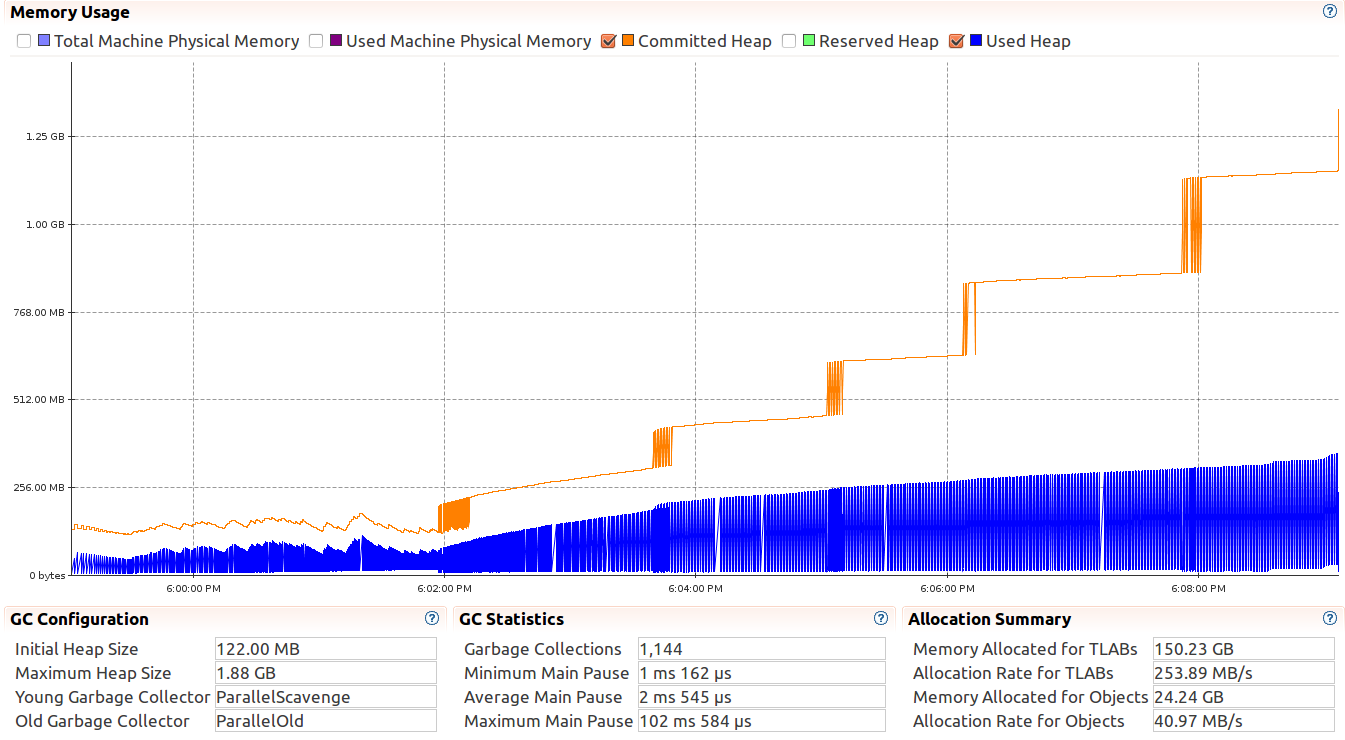
\includegraphics[width=0.95\linewidth]{img/stage_2/memory.png}
		%		\caption{Test}
		\label{fig:mem2}
	\end{figure}
	\newpage
	
	Дамп \#3
	\begin{figure}[h!] % \ContinuedFloat
		\centering
		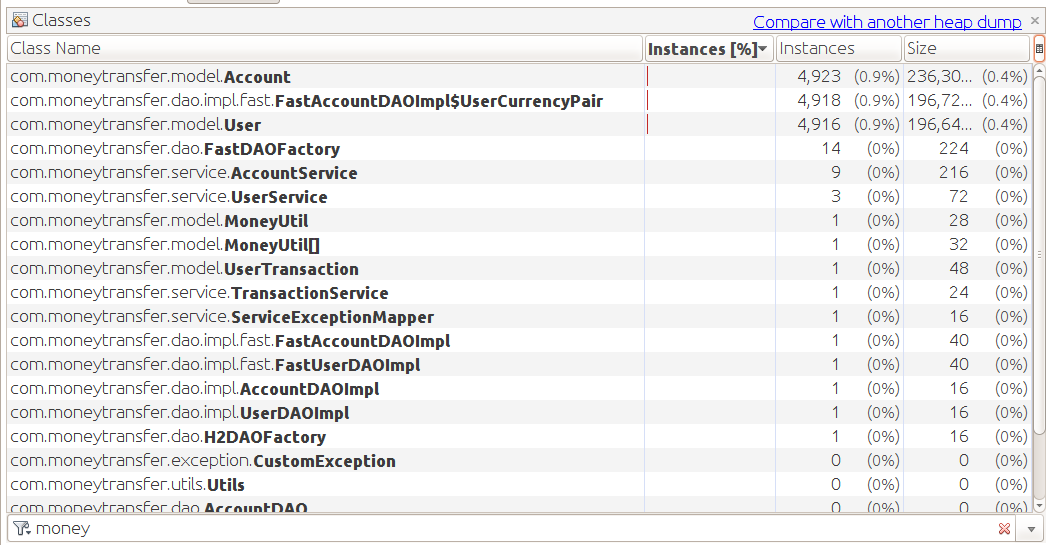
\includegraphics[width=0.75\linewidth]{img/stage_2/dump3.png}
		%		\caption{Test}
		\label{fig:dmp32}
	\end{figure}
	
	Судя по дампу объекты создаются и уничтожаются правильно, за исключением \texttt{FastDAOFactory}.
	
	\item \textit{Как часто происходит сборка мусора?}
	
	За время эксперимента произошла 1144 раз. Средняя пауза 2 ms 545 us, максимальная 102 ms 584 us. 
	
	\item \textit{Сколько в среднем выполняется запуск сценария 1, как быстро увеличивается это время?}
	
	Текущее время выросло с 0.04 с до  0.57 с за 11200 выполнений сценария 1. 
	По сравнению с предыдущим этапом, общая производительность немного ниже.
	
	\begin{figure}[h!] % \ContinuedFloat
		\centering
		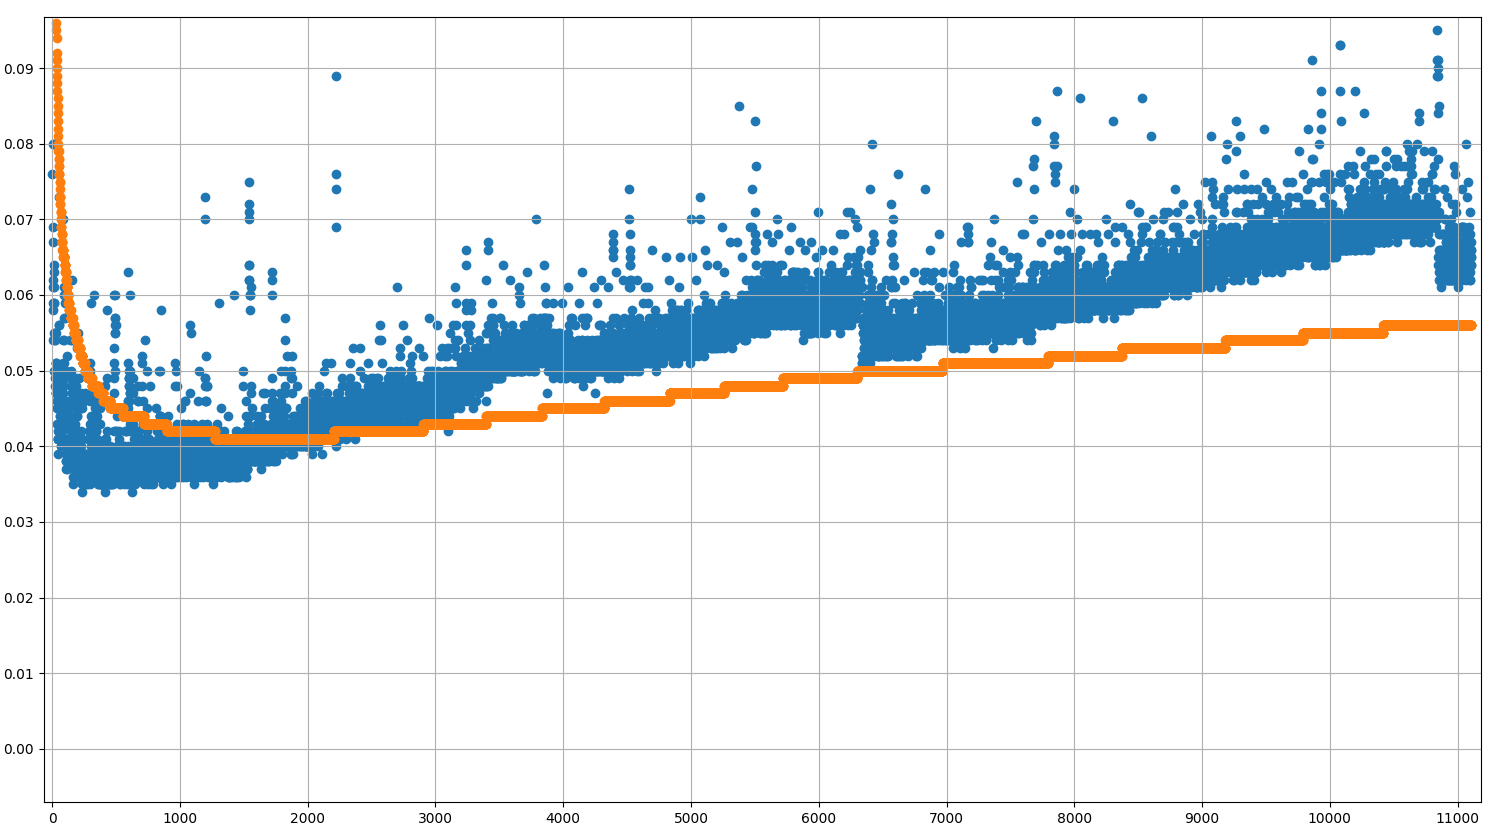
\includegraphics[width=0.95\linewidth]{img/stage_2/pyplot.png}
		\label{fig:pyplot2}
	\end{figure}
	
	\newpage
	\item \textit{Какие операции из значимых (т.е. без учёта работы системных функций, в т.ч. веб сервера) занимают больше всего процессорного времени?}
	
	Чаще всего CPU обрабатывает те же методы, что и на предыдущем этапе.
	
	\begin{figure}[h!] % \ContinuedFloat
		\centering
		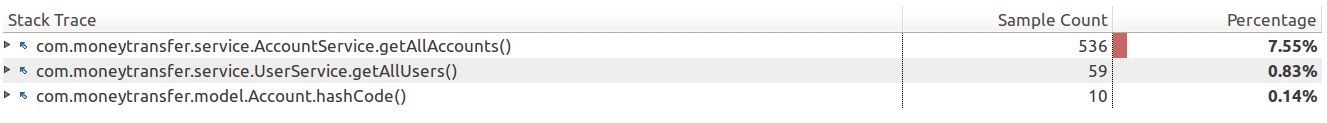
\includegraphics[width=0.95\linewidth]{img/stage_2/hotmethods.png}
		\label{fig:hotmethods2}
	\end{figure}
	
	\item \textbf{ВЫВОДЫ СТАДИИ 2}
	\begin{enumerate}
		\item Изменения позволили снизить загрузку процессора ещё на 3-4\%
		\item Потребление памяти изменилось незначительно
		\item Общая производительность ухудшилась на несколько процентов
		\item in memory СУБД обладает не худшими характеристиками по сравнению с самописным хранилищем на \texttt{HashMap}   
	\end{enumerate}
\end{itemize}


\end{document}